%------------------------------------------------------------
%
\documentclass[landscape, notitlepage]{article}%
%Options -- Point size:  10pt (default), 11pt, 12pt
%        -- Paper size:  letterpaper (default), a4paper, a5paper, b5paper
%                        legalpaper, executivepaper
%        -- Orientation  (portrait is the default)
%                        landscape
%        -- Print size:  oneside (default), twoside
%        -- Quality      final(default), draft
%        -- Title page   notitlepage, titlepage(default)
%        -- Columns      onecolumn(default), twocolumn
%        -- Equation numbering (equation numbers on the right is the default)
%                        leqno
%        -- Displayed equations (centered is the default)
%                        fleqn (equations start at the same distance from the right side)
%        -- Open bibliography style (closed is the default)
%                        openbib
% For instance the command
%           \documentclass[a4paper,12pt,leqno]{article}
% ensures that the paper size is a4, the fonts are typeset at the size 12p
% and the equation numbers are on the left side
%
\usepackage{graphicx,showexpl,listings}
\usepackage{tikz}
\usetikzlibrary{shapes.symbols, 
		shapes.geometric,
		arrows,
		decorations.pathmorphing,
		positioning,
		backgrounds,
		fit}
%-------------------------------------------

\begin{document}
\pagenumbering{gobble}
\topmargin=-10pt
\footskip=0pt
\center\small{Component Interaction: \large{SQW Data System}}

\begin{tikzpicture}[place/.style={
					circle,
					draw=blue!50,fill=blue!20,thick,
					inner sep=0pt,minimum size=6mm},
			component/.style={
					rectangle,
					draw=black!50,fill=blue!20,thick,
					minimum width=3cm,
					inner sep=10pt},
			innercomponent/.style={component, 
						       dotted, 
						       minimum width=0, inner sep=5pt},
			outsys/.style={component, fill=black!20},
			unused/.style={component,fill=black!10,dotted},
			inlay/.style={
					rectangle,
					draw=black!60,thick,dotted,
					minimum size=15mm,
					inner sep=2pt},
			%every label/.style=red,
			tinyfont/.style={font=\it\tiny},
			smallfont/.style={font=\it\small},
			elab text/.style={tinyfont,align=center},
		      elab/.style={above,elab text},
			elabb/.style={below,tinyfont,elab text},
			elabs/.style={above,sloped,elab text},
			elabbs/.style={below,sloped,elab text},
			end point/.style={circle,fill=red!30,draw=black!30,thick,
						 inner sep=1pt,
						 minimum size=5mm},
			database/.style={cylinder,draw,align=center,
						 fill=green!20,
						 aspect=.10,
						 minimum size=1cm,
						 minimum height=1cm+20pt,
						 inner sep=2pt,
						 shape border rotate=90},
			multipledb/.style={database,smallfont},
			returning/.style={dotted,bend angle=20,bend left},
			this is/.style=dotted,
			ital/.style={font=\itshape},
			subsys/.style={fill=red!10,ital,inner sep=5pt},
			bend angle=20,
			pre/.style={<-,shorten <=1pt,>=stealth',semithick},
			post/.style={->,shorten >=1pt,>=stealth',semithick}]
%% -------------- GRID ----------------------------------------- %%
	\path[help lines, blue!20, draw] grid (12,12);

%% --------------- SPEED LAYER ------------------------------ %%
\node [component, xshift=20pt, yshift=-5pt] (streamproc) at (2, 11) {Stream Processor};

\node [above=of streamproc,xshift=20pt,yshift=-1cm,ital] (speedtitle) {Speed Layer};
\node [database,right=of streamproc,xshift=10pt] (speeddb) {Recent Data\\R/W}
	edge [pre] node [elab] {read/write} (streamproc);

%% --------------- GATEWAY ------------------------------ %%
\node [component, below=of streamproc, xshift=20pt,yshift=-10pt] (ghreads) {Read Handler}
	edge [post, bend left] node [elabs] (aggend1) {sql command} (speeddb);

\node [below=of ghreads,xshift=-5pt,yshift=20pt,ital] (gtitle) {Gateway};

\node [component, below=of ghreads,xshift=-20pt, yshift=0cm] (ghwrites) {Write Handler}
	edge [pre, bend angle=45, bend left] node [elabs,xshift=10pt] {process write data} (streamproc);

\node [innercomponent,below=of ghwrites,xshift=27pt,yshift=15pt]	
									(gser) {Serializer}
	edge [pre,bend right] node [elab,xshift=17pt,yshift=-5pt] {toBytes(data)} (ghwrites);

%% ---------------- CLIENT FIGURES ------------------------ %%
\node [left=of streamproc,xshift=10pt, yshift=-10pt] (write) 
		{ 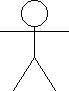
\includegraphics[width=0.4cm]{../img/stick.png}}
	edge [post, dotted, xshift=-3pt] (streamproc);
\node [below=of write,tinyfont,yshift=25pt] {Update request};

\node [ left=of ghreads,xshift=-10pt, yshift=-20pt] (read) 
		{ 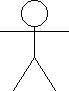
\includegraphics[width=0.4cm]{../img/stick.png}}
	edge [post, dotted, xshift=-3pt] (ghreads);
\node [below=of read,tinyfont,yshift=25pt] {Data request};

%% --------------- SERVING LAYER ------------------------------ %%
\node [component, right=of ghreads,xshift=0pt,yshift=-20pt] (servqh) {Query Engine}
	edge [pre, bend left] node [elabbs] (aggend2) {custom query} (ghreads);

\node [below=of aggend1,xshift=15pt,yshift=12pt] {\itshape{merged}}
	edge [dotted,thick] (aggend1)
	edge [dotted,thick] (aggend2);

\node [multipledb, right=of servqh,xshift=-8pt,yshift=0cm] (servdb1) {Query $1$ Store};

\node [inlay, below=of servqh, yshift=20pt,xshift=5pt] {indexer};

\node [multipledb, below=of servdb1,xshift=0pt,yshift=20pt] (servdbn) {Query $n$ Store}
	edge[dashed] (servdb1);

\node [above=of servqh,xshift=30pt,yshift=-15pt,ital] (servtitle) {Serving Layer};

	%% ----- phantom anchor nodes for db background border end points
\node [below=of servdbn,xshift=0pt,yshift=1cm+3pt] (servdbend1) {};
\node [left=of servdbn,xshift=1cm+2pt,yshift=30pt] (servdbend2) {};


%% --------------- BATCH LAYER ------------------------------ %%
	%% ----------- WRITES ------------------------%%
\node [innercomponent, below=of gser,xshift=10pt,yshift=10pt] (bdeser) {Deserializer};

\node [component, below left=of bdeser,xshift=1cm+10pt,yshift=20pt] (bwriter) {Writer}
	edge [post, bend right] node [elab, xshift=20pt,yshift=-8pt] {getData(bytes)} (bdeser)
	edge [pre] node [elab, xshift=-15pt,yshift=8pt] {write(bytes)} (ghwrites);

\node [component, below=of bwriter,yshift=0pt] (bformatter) {Formatter}
	edge [pre] node [elab,xshift=-20pt,yshift=-10pt] {format data\\and save} (bwriter);

\node [database, right=of bformatter,yshift=-5pt] (bfile) {File System\\HDFS}
	edge [pre] node [elab,xshift=-2pt] {write} (bformatter);

	%% ------------ SNAPSHOT ----------------------%%
\node [component, right=of bfile,xshift=-1cm+20pt,yshift=30pt] 
							(bassembler) {Datalog};

\node [innercomponent, above=of bassembler, xshift=2pt,yshift=-4pt+4pt,align=center]
							(bcommand) {Data Snapshot\\Command}
	edge [post] node [elab, xshift=-15pt] {get job} (bassembler)
	edge [pre,returning] node [elab,xshift=5pt] {job} (bassembler)	
	edge [post,bend left] node [elab, xshift=-12pt,
					 yshift=-15pt] {switch} (servdbend2)
	edge [post, bend angle=45, bend left]
			 node [elab, xshift=-7pt,yshift=-1.5cm] 
				{wipe out\\records before\\snapshot timestamp} (speeddb);

\node [component, below right=of bassembler,xshift=-2cm,yshift=20pt] 
								(mapreduce) {Map-Reduce}
	edge[pre,bend right] node [elab,xshift=7pt] {run job} (bcommand)
	edge[pre, bend left, dotted] node [elab,xshift=-20pt, yshift=-3pt] 
								{has defined} (bassembler)
	edge[post] node [elabbs] {read all records} (bfile)
	edge[post, bend right] node [elab,xshift=17pt] {populate\\snapshot} (servdbend1);

\node [right=of bwriter,xshift=20pt,yshift=0pt, ital] (btitle) {Batch Layer};

	%%  ------------------------- demarcation b/w reads and writes in batch layer----%%
\draw[dotted,thick] (5,0) -- (6,4.6);

%% ------------------------------ COMMENTS -------------------------------- %%
\node [right=of speeddb,ital,smallfont,align=left,yshift=15pt] {Transactionsl RDBMS}
	edge  (speeddb);

\begin{pgfonlayer}{background}
	\node [subsys, 
			fit=(streamproc) (speeddb)]
		{};
\end{pgfonlayer}

\begin{pgfonlayer}{background}
	\node [subsys, black!5,
			fit=(gser) (ghwrites) (ghreads)]
		{};
\end{pgfonlayer}

\begin{pgfonlayer}{background}
	\node [subsys, blue!10,
			fit= (servtitle) (servqh) (servdb1) (servdbn)]
		{};
\end{pgfonlayer}

\begin{pgfonlayer}{background}
	\node [dotted,thick,draw,inner sep=4pt,
			fit=  (servdb1) (servdbn)]
		(servdbborder){};
\end{pgfonlayer}

\node [above=of servdb1,ital,smallfont,align=left] {Fast, Read-Only\\NoSQL databases}
	edge [ yshift=2pt] (servdbborder);

\begin{pgfonlayer}{background}
	\node [subsys, yellow!30,
			fit=  (bwriter) (bdeser)  (bformatter) (bfile) (bassembler) (mapreduce)]
		{};
\end{pgfonlayer}
\end{tikzpicture}
\end{document}